\subsection{Frank-Wolfe, the conditional gradient algorithm}
%WILL blabla
\subsection{Away steps Frank-Wolfe}
When the minimizer of the objective function lies at the boundary of the domain,
after a number of iterations, the duality gap starts to stagnate.\\ As a result
of the strong dependency of the immediate iterate on previously accumulated
atoms in the active set, as it approaches to boundary, the F-W algorithm starts
to zig-zag around the descent direction as can be seen in figure 2.\\
% \begin{algorithm}[tb]
%    \caption{Away-steps Frank-Wolfe}
%    \label{alg:example}
\begin{algorithmic}
    \STATE {Let $x_{0}\in\mathcal{A}$ and $S_{0}:=\{x_{0}\}$}\\
    \FOR {$t=0...T$}{
        \STATE{Let $s_{t}:= LMO_{\mathcal{A}}(\nabla f(x_{t}))$ and $d^{FW}_{t}:= s_{t}- x_{t}$}\\
        \STATE{Let $v_{t}\in \underset{v\in S_{t}}{\textit{argmax}}\langle\nabla f(x_{t}), v\rangle$ and $d^{A}_{t}:= x_{t}- v_{t}$}\\
        \STATE {\textbf{if} $g^{FW}_{t}=\langle-\nabla f(x_{t}),
d^{FW}_{t}\rangle\leq \epsilon$ \textbf{then return} $x_{t}$}\\ \STATE
{\textbf{if} $\langle-\nabla f(x_{t}), d^{FW}_{t}\rangle\geq \langle-\nabla
f(x_{t}), d^{A}_{t}\rangle$\quad\textbf{then}}\\
\STATE{\quad\quad\quad$d_{t}=d^{FW}_{t}$ and $\gamma^{max}=1$}\\
\STATE{\textbf{else}}\\
        \STATE{\quad\quad\quad $d_{t}=d^{A}_{t}$ and
$\gamma^{max}=\frac{\alpha^{(t)}_{v_{t}}}{1-\alpha^{(t)}_{v_{t}}}$}\\
\STATE{Line-search: $\gamma_{t}\in\underset{\gamma}{argmin}f(x_{t}+\gamma
d_{t})$}\\ \STATE{Update $x_{t}= x_{t}+\gamma_{t}d_{t}$}\\ } \ENDFOR
\end{algorithmic}
%\end{algorithm}
% \begin{figure}
%   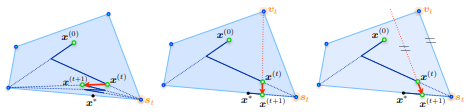
\includegraphics[width=\linewidth]{fig2.png}
%   \caption{(left) The FW algorithm zig-zags when the solution $x$ lies on the
% boundary. (middle) Adding the possibility of an away step attenuates this
% problem. (right) As an alternative, a pairwise FW step.}
%   \label{fig:Away steps}
% \end{figure}

To address this issue an improved variant of F-W named \textbf{Away-steps
Frank-Wolfe} adds the possibility of moving away (by removing a fraction of) a
maximizer of the $LMO_{\mathcal{S_{t}}}$ in the active set. While this slows
down each iteration it should be noted that the added step is easier than
$LMO_{\mathcal{A}}$ given that we maximize over a subset of $\mathcal{A}$.
Furthermore, given that this variant converges linearly, the algorithm
progresses in a fewer number of iterations in the descent direction, making it
much faster than the original F-W.
\subsection{Block Coordinate Frank Wolfe}
\subsection{Structured SVM context}
Given a training set $\mathcal{D}=\{(x_i,y_i)\}_{i=1}^n$ where $y \in
\mathcal{Y}$ is a multi-label output, and a feature map
$\phi:\mathcal{X}\times\mathcal{Y}\longrightarrow \mathbb{R}$, which encodes a
similarity measure between $\mathcal{X}$ and $\mathcal{Y}$, such that if $y_{i}$
is the ground truth (target) for an input $x_{i}$, then
\begin{equation*}
\begin{aligned}
    &\forall y\in\mathcal{Y}\texttt{\symbol{92}}\{y_{i}\}\quad\textit{we
have}\quad \psi_{i}(y) = \phi(x_{i},y_{i})- \phi(x_{i},y) > 0
\end{aligned}
\end{equation*}
The aim is to construct an accurate linear classifyer, $h_{w}(x)=
\underset{y\in\mathcal{Y}(x)}{\textit{argmax}}\langle w, \phi(x,y)\rangle$.\\ To
learn $w$, consider the task loss
$L:\mathcal{Y}\times\mathcal{Y}\longrightarrow\mathbb{R}_{+}$, where
$L(y,y\prime)= 0 \Longleftrightarrow y= y\prime$. \\

The $n$-slack formulation of the problem would be,
\begin{equation*}
\begin{aligned}
    &\underset{w,\xi}{\textit{max}}\quad\frac{\lambda}{2}||w||^{2}+ \frac{1}{n}\sum_{i=1}^{n}\varepsilon_{i}\\
    &\textit{s.t.}\quad \langle w, \psi_{i}(y)\rangle \geq L(y_{i},y)-
\varepsilon_{i},\quad\forall i ,\forall y\in\mathcal{Y}(x)=\mathcal{Y}_{i}
\end{aligned}
\end{equation*}
\textit{Problems:} (1) The zero-one loss is not differentiable and (2) we have
an exponential number of constraints.\\ \textit{Solutions:} (1) Minimizing an
upper bound to the task loss gives us a worst case guarantee.\\


Consider the \textbf{max oracle}, $\Tilde{H}=
\underset{y\in\mathcal{Y}_{i}}{\textit{max}}$ $\underbrace{L_{i}(y)- \langle w,
\psi_{i}(y)\rangle}_{= H_{i}(y,w)\quad\textit{the hinge loss}}$.\\ (2) The
exponential number of constraints are replaced by $n$ piecewise linear ones. \\

\textbf{Proposition.} The max oracle is a convex upper bound to the task loss.\\
\textit{Proof.} The maximum of two convex (linear) functions is convex, and
\begin{equation*}
\begin{aligned}
    &L(y_{i},h_{w}(x_{i})) \leq L(y_{i},h_{w}(x_{i})) + \underbrace{\langle w, \psi_{i}(y)\rangle}_{\geq 0 \textit{ by definition}} \\
    &\quad\quad\leq \underset{y\in\mathcal{Y}_{i}}{\textit{max}} L_{i}(y)- \langle w, \psi_{i}(y)\rangle
\end{aligned}
\end{equation*}
Thus learning $w$ amounts to the unconstrained problem,
\begin{equation*}
\begin{aligned}
    &\underset{w}{\textit{max}}\quad\frac{\lambda}{2}||w||^{2}+ \frac{1}{n}\sum_{i=1}^{n}\Tilde{H}_{i}(w)
\end{aligned}
\end{equation*}
\subsubsection{BCFW variant in the structured SVM setting}
Due to the exponential number of dual variables in the structured SVM setting,
classical algorithms, like projected gradient are intractable. \\
Stochastic subgradient methods, on the other hand, achieve a sublinear
convergence rate while only requiring a single call to the maximization oracle
every step. They are nonetheless very sensitive to the sequence of stepsizes and
it is unclear when to terminate the iterations. \\

Frank-Wolfe methods address these problems by giving an adaptive stepsize
$\gamma= \frac{2}{k+2}$ and a computable duality gap while still retaining a
sublinear convergence rate. Moreover, despite the exponential number of
constraints, the algorithm has sparse iterates alleviating the memory issues
which come with the exponential number of dual variables.\\
\textbf{Note.} The main idea here, is that the linear subproblem in Frank-Wolfe
and the loss augmented decoding of the structured SVM are equivalent. \\

\textit{Proof of the equivalence.} The objective function being differentiable
and convex, if we are at a point $\alpha$ such that $f(\alpha)$ is minimized
along each coordinate axis, then $\alpha$ is
a global minimizer. Therefore,

\begin{equation*}
\begin{aligned}
    &\underset{s\in\mathcal{M}}{\textit{min}}\langle s, \nabla f(\alpha)\rangle
= \sum_{i}\underset{s_{i}\in\Delta_{|\mathcal{Y}_{i}|}}{\textit{min}}\langle
s_{i}, \nabla_{i} f(\alpha)\rangle
\end{aligned}
\end{equation*}
Moreover, with
\begin{equation*}
\begin{aligned}
   &w=A\alpha, A=\Big[\frac{1}{n\lambda}\psi_{1}(y)...\frac{1}{n\lambda}\psi_{\sum_{i}|\mathcal{Y}_{i}|}(y)\Big]\\
   &\textit{and}\quad b=\Big(\frac{1}{n}L_{i}(y)\Big)_{i\in\big[n\big],y\in\mathcal{Y}_{i}}
\end{aligned}
\end{equation*}
The gradient of the dual would be,
\begin{equation*}
\begin{aligned}
    &\nabla f(\alpha)= \nabla\Big[\frac{\lambda}{2}||A\alpha||^{2}- b^{T}\alpha\Big] = \lambda A^{T}A\alpha- b\\
    &= \lambda A^{T}w- b= \frac{1}{n}H_{i}(y,w)\\
    &\underset{y_{i}\in\mathcal{Y}_{i}}{\textit{max}}\quad\tilde{H}_{i}=
  -\underset{y_{i}\in\mathcal{Y}_{i}}{\textit{min}}\quad\tilde{H}_{i} =
  \underset{y_{i}\in\mathcal{Y}_{i}}{\textit{min}}\quad L_{i}- \langle w,
  \psi_{i}\rangle\\ &=
  \underset{s_{i}\in\Delta_{|\mathcal{Y}_{i}|}}{\textit{min}}\langle s_{i},
  \nabla_{i} f(\alpha)\rangle\\
\end{aligned}
\end{equation*}
Thus we can see that, if $n=$ size of the training data, one Frank-Wolfe step is equivalent to $n$ calls to the maximization oracle.
\begin{algorithmic}
   \STATE Let $\alpha\in\mathcal{M}$
    \STATE {Let $w^{0}= 0$, $l^{0}= 0$}\\
    \FOR{$k=0, \dots, K$}
      \FOR{$i=1, \dots, n$}
        \STATE {Solve $y_{i}^{*}=\underset{y_{i}\in\mathcal{Y}_{i}}{\max} H_{i}(y,w^{k})$//
        \STATE {Let $w_{s}=
\sum_{i=1}^{n}\frac{1}{n\lambda}\psi_{i}(y_{i}^{*})$, and $l_{s}=
\frac{1}{n}\sum_{i=1}^{n}L_{i}(y_{i}^{*})$}\\ \STATE {Let $\gamma=
\frac{\lambda(w^{k}-w_{s})^{T}w^{k}- l^{k}+ l_{s}}{\lambda||w^{k}-w_{s}||^{2}}$,
and clip to $[0,1]$}\\ \STATE {Update $w^{k+1}= (1-\gamma)w^{k}+ \gamma w_{s}$,
and $l^{k+1}= (1-\gamma)l^{k}+ \gamma l_{s}$}
    }
   \ENDFOR
   \ENDFOR
\end{algorithmic}

Unlike stochastic subgradient and stochastic methods in general, classical
Frank-Wolfe requires one call for each training example at each iteration. For
large datasets, this can get unpractical.\\ Hence the stochastic variant of
Frank Wolfe, \textbf{Block Coordinate Frank Wolfe (BCFW)}.\\



%%% Local Variables:
%%% mode: latex
%%% TeX-master: "mainProject"
%%% End:
